\documentclass[sigconf]{acmart}

\usepackage{booktabs}
\usepackage{hyperref}
\usepackage{listings}
% * <marc.vornetran@gmail.com> 2018-03-02T13:58:29.061Z:
%
% ^.
\usepackage{color}

\newcommand\todo[1]{\textbf{\textcolor{red}{#1}}}

\definecolor{lightgray}{rgb}{.9,.9,.9}
\definecolor{darkgray}{rgb}{.4,.4,.4}
\definecolor{purple}{rgb}{0.65, 0.12, 0.82}

\lstdefinelanguage{JavaScript}{
  keywords={do, if, in, for, let, new, try, var, case, else, enum, eval, null, this, true, void, with, await, break, catch, class, const, false, super, throw, while, yield, delete, export, import, public, return, static, switch, typeof, default, extends, finally, package, private, continue, debugger, function, arguments, interface, protected, implements, instanceof},
  morecomment=[l]{//},
  morecomment=[s]{/*}{*/},
  morestring=[b]',
  morestring=[b]",
  ndkeywords={class, export, boolean, throw, implements, import, this},
  keywordstyle=\color{blue}\bfseries,
  ndkeywordstyle=\color{darkgray}\bfseries,
  identifierstyle=\color{black},
  commentstyle=\color{purple}\ttfamily,
  stringstyle=\color{red}\ttfamily,
  sensitive=true
}

\lstset{
   language=JavaScript,
   extendedchars=true,
   basicstyle=\footnotesize\ttfamily,
   showstringspaces=false,
   showspaces=false,
   tabsize=2,
   breaklines=true,
   showtabs=false,
   captionpos=b
}


\settopmatter{printacmref=false}
\renewcommand\footnotetextcopyrightpermission[1]{} % removes footnote with conference information in first column
\pagestyle{plain} % removes running headers

\begin{document}
\title{Identification Rumble}
\subtitle{Increasing interaction between visitors and World War II dilemmas in the Dutch Resistance Museum}

\author{Maaike Koolbergen}
\affiliation{
  \institution{University of Amsterdam}
  \city{Amsterdam}
  \country{The Netherlands}
}
\email{maaikekoolbergen@gmail.com}

\author{Gokie Wiegers}
\affiliation{
  \institution{University of Amsterdam}
  \city{Amsterdam}
  \country{The Netherlands}
}
\email{gokie.wiegers@gmail.com}

\author{Jerom Fernig}
\affiliation{
  \institution{University of Amsterdam}
  \city{Amsterdam}
  \country{The Netherlands}
}
\email{jeromfernig@gmail.com}

\author{Marc Vornetran}
\affiliation{
  \institution{University of Amsterdam}
  \city{Amsterdam}
  \country{The Netherlands}
}
\email{marc.vornetran@gmail.com}


\begin{abstract}
The main exhibition of the Dutch Resistance Museum in Amsterdam about the Netherlands in World War II illustrates personal experiences of Dutch citizens during the occupation but has been largely left unchanged for almost two decades. The museum has asked Master of Science students from the University of Amsterdam to develop one or more interactive museum exhibits that present twelve main dilemmas Dutch citizens faced during the occupation of the Netherlands by Nazi Germany. Through user-centered design and extensive iteration, an interactive and engaging experience is proposed. This paper presents the design, development and use of the interactive museum experience: \textit{Identification Rumble}. 
\end{abstract}

\keywords{Tangible interactions, interaction design, user experience, smart replica, interactive museum exhibit, Dutch Resistance Museum}

\maketitle
\section{Introduction}
The goal of this review paper is to establish a broad birds-eye view on the following areas within games: Design frameworks, mechanics, story, and artificial intelligence.
In the beginning the three main design frameworks are covered chronologically.
Published in 2004 the Mechanics-Dynamics-Aesthetics framework (MDA) by Hunicke et al. \cite{Hunicke2004} set out to establish a common language to reason about games and analyze them from different perspectives (Section \ref{sec:mda}.
The elemental tetrad by Schell in 2008 \cite{Schell2014} picks up the concepts of mechanics and aesthetics (Section \ref{sec:elemental-tetrad}).
It introduces story and technology and puts the components into relation.
This paper continues by covering mechanics (Section \ref{sec:mechanics} and story (Section \ref{sec:story}) as identified by Schell in greater detail.
He argues that while it is difficult to create a unified taxonomy due to the hidden complexity of mechanics it is still worthwile to work towards a common understanding.
Mechanics are the core of every game and need to be understood to reason about it.
Interactive storytelling is a new concept introduced by videogames which proves to be inherently difficult to implement.
Paying attention to traditional storytelling and following guidelines for the creation of the feeling of freedom helps to produce interesting experiences using interactive storytelling.
Finally, the last section of the paper provides insights into the ten research areas of AI in games as Yannakakis and Togelius identified them in 2015 (Section \ref{sec:ai}).
It also explores the application of AI planning to computational narratives in the article by Porteous et al.\cite{Porteous2010} (Section \ref{sec:search-and-planning}).

\section{MDA Framework} \label{sec:mda}
Hunicke et al. (2004) \cite{Hunicke2004} published their Mechanics-Dynamics-Aesthetics (MDA) framework as a formal approach towards establishing a clear understanding of games.
It aims to connect the fields of game design, development, criticism, and technical research.
Creating a common vocabulary allows to reason about game artifacts and iteratively improve them.

As videogames grow more and more complex it becomes increasingly difficult to keep track of all aspects shaping a game and influencing each other.
Small changes to one area might propagate through different structures and change gameplay in unexpected ways.
This emphasizes the need for an abstract, clear view on games as a coherent system.

The MDA framework (Figure \ref{fig:mda}) starts by breaking apart the consumption of games into: (1) Rules, (2) system, and (3) ``fun''.
It consequently translates these components into their design counterparts: (1) Mechanics, (2) dynamics, and (3) aesthetics.
Mechanics refer to the bare-bone data representations and algorithms at the heart of a game.
At run-time dynamics are produced by the underlying mechanics through player inputs and subsequent dynamic outputs.
Finally, the previous components results in aesthetics which describe the emotional responses of players.
This chain already indicates that changes to the basic mechanics will propagate through dynamics and emerge as different gameplay experiences.

\begin{figure}[H]
    \centering
    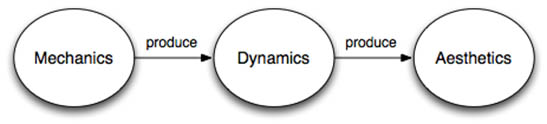
\includegraphics[width=8cm]{assets/mda.jpg}
    \caption{MDA framework\protect\footnotemark}
    \label{fig:mda}
\end{figure}
\footnotetext{\url{http://www.firstpersonscholar.com/a-working-theory-of-game-design}, Accessed: 02-03-2018}

As MDA splits games into three components they can be used as views on different layers of games.
These views enable looking at games from both a designer's perspective but also from the player's perspective.
Players naturally view games from the opposite direction: Aesthetics define the experience, which are created by observable dynamics, which in turn are the result of mechanics.
The following sections discuss the components of MDA starting from a player's perspective which is in line with experience-driven design \cite{Hunicke2004}.

\subsection{Aesthetics}
The authors defined a taxonomy of eight elements to describe the aesthetics of a game: (1) Sensation (sense-pleasure), (2) fantasy (make-believe), (3) narrative (drama), (4) challenge (obstacle course), (5) fellowship (social framework), (6) discovery (uncharted territory), (7) expression (self-discovery), and (8) submission (pastime).
This taxonomy aims to extend the previously limited vocabulary with meaningful categories.
Games are certainly not limited to only one or a subset of these aesthetics.
Instead they tend to emphasize each aesthetic to a different degree.

\subsection{Dynamics}
Dynamics are responsible for producing different aesthetic experiences.
It is useful for designers to understand which types of dynamics influence various aesthetics areas.
As an example (4) challenge can be induced by limiting time, placing obstacles and letting the player face opponents.
Conceptualizing models of gameplay dynamics provides insights into their behavior and potentially highlights deficiencies.
This is especially useful for probabilities as common misconceptions might lead sub-optimal experiences.

\subsection{Mechanics}
Mechanics span the player's affordances (actions, controls) as well as the game space itself (worlds, objects, characters).
The sum of basic mechanics supports the dynamics during gameplay.
This is commonly visible as emergent behavior in games where players attempt to fool their opponents or use specific strategies to their own advantage.
Carefully modifying the underlying mechanics of a game allows designers to influence the resulting dynamics.
The ``Mario Kart'' series by Nintendo is a prominent example featuring mechanics initially designed to help players on lower ranks to overtake their opponents more easily.
Players are able to collect items throughout the course; their strength and overall usefulness greatly depends on the current rank of a player.
However, most of the time this item distribution results in an undesired dynamic during gameplay.
As players in the back are rewarded with powerful, chaotic items they tend to entangle their nearby opponents in ongoing fights.
Meanwhile, players at the top of the ranking enjoy relatively weak attacks and can defend their position more easily.
\section{Elemental Tetrad} \label{sec:elemental-tetrad}
\citeauthor{Schell2014} created the \textit{elemental tetrad} in 2008 in the first edition of his book as a design tool to dissect games into their four basic components (Figure \ref{fig:elemental-tetrad}.
The four components include: (1) Mechanics, (2) story, (3) aesthetics, and (4) technology.
Figure \ref{fig:elemental-tetrad} visualizes the classification of aesthetics as being the most visible, with mechanics and story taking the middle ground, and finally technology being the less visible layer.

\begin{figure}[H]
    \centering
    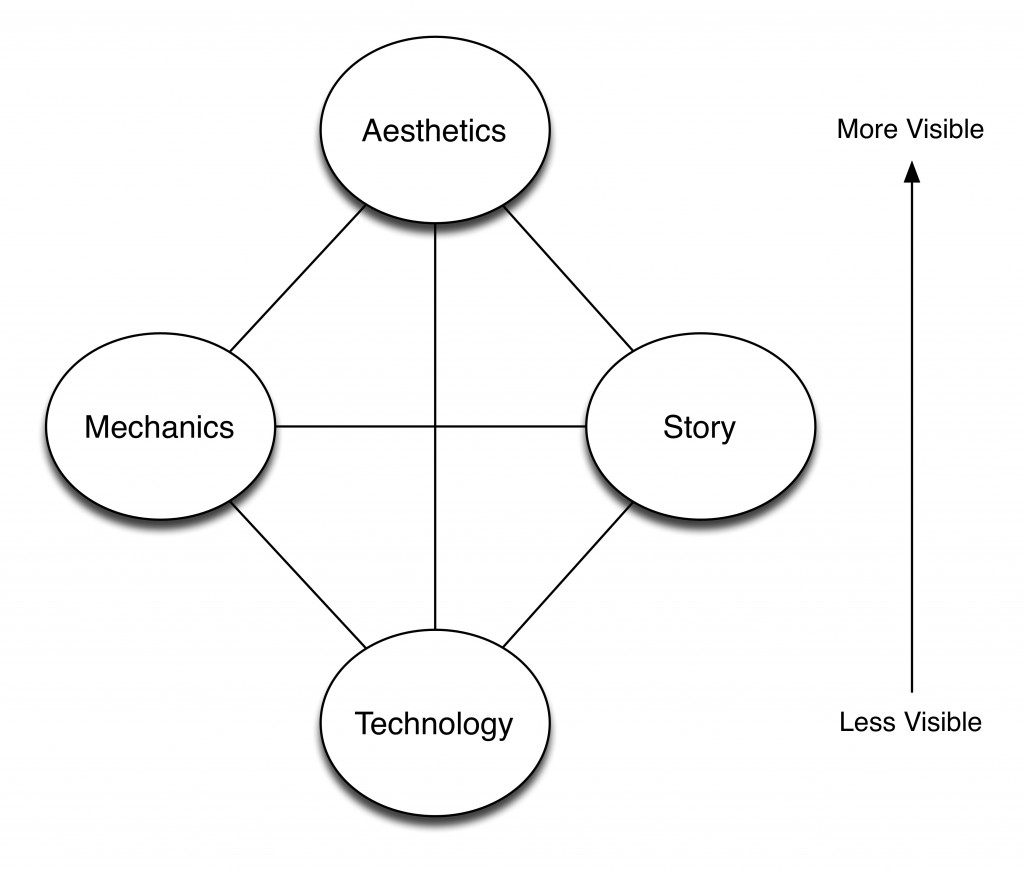
\includegraphics[width=8cm]{assets/elemental-tetrad.jpg}
    \caption{Elemental Tetrad according to Schell\protect\footnotemark}
    \label{fig:elemental-tetrad}
\end{figure}
\footnotetext{\url{http://www.firstpersonscholar.com/a-working-theory-of-game-design}, Accessed: 02-03-2018}

Mechanics (Section \ref{sec:mechanics}) and story (Section \ref{sec:story}) according to \citeauthor{Schell2014} are covered in greater detail in this paper.
Aesthetics cover how a player's senses perceive a game: Visuals, sounds, smells, tastes, and haptic feeling.
Due to their apparent nature they are a crucial part of the experience.
The MDA framework (Section \ref{sec:mda}) and MTDA+N framework (Section \ref{sec:mtda+n}) discuss aesthetics in detail.
Technology refers to all physical and virtual media allowing to play a game.
This spans simple materials such as pen and paper as well as digital software powering videogames.

\subsection{Mechanics} \label{sec:mechanics}
In his work \citeauthor{Schell2014} discerns seven distinct mechanics which define what a game is in its core.
They can be seen as the skeletal frame of a game behind the curtain of aesthetics, technology and storytelling.
Game designers should be able to look behind this curtain and identify the main mechanics making up a specific game.
He argues that while their is no single standard taxonomy due to the inherent complexity and hidden structures it is worthwhile to work towards a common understanding.
Definitions should avoid both too much simplification and excessive precision.
In the end the classifications should work towards providing useful insights into games for designers \cite{Schell2014}.

\subsubsection{Space} \label{sec:space}
Thinking about the \textit{space} of a game requires an abstract, mathematical view which blanks out any visual aesthetics.
A game's space describes all possible places and their connection to each other.
They feature three main characteristics \cite{Schell2014}:
\begin{itemize}
    \item Discrete or continuous
    \item Number of dimensions
    \item Bounds and connections
\end{itemize}
\textit{Discrete} spaces are restricted to a finite number of places.
Board games commonly have this characteristic; even though pieces can be freely placed within the area of 2D boards (sometimes 3D) only a set of places carries meaning for the mechanics of the game.
Conversely, \textit{continuous} space can also be restricted in terms of its dimensions but elements are placed freely at any position.
Pong\footnote{\url{https://en.wikipedia.org/wiki/Pong}, Accessed: 01-03-2018} is a good example for a 2D playing field with continuous movement.
It recreates top-down table tennis with paddles on either side and a ball moving back and forth.
Both paddles are locked into vertical bounds but can have any arbitrary position within.

The previous characteristic already touched upon the \textit{dimensionality} of games.
Naturally, two dimensions (2D) and three dimensions (3D, reality) come to mind.
Information state can also be represented in an abstract space model.
Even when a game, like quiz games, might not feature a dimensional world the state of players exists in zero dimensional spaces.

Finally, the third characteristic is concerned with \textit{bounding areas} in spaces or if they are \textit{connected}.
The contrast is visible when thinking of bounded board games versus Pong again. 
Various places in a board game have limited areas where pieces can be placed.
Within this area positions carry the same meaning; borders to neighboring fields create a pathway through the game.
In Pong the areas are connected and allow for free movement of elements.

With these characteristics in mind complexity increases when nesting multiple spaces.
Nested spaces are not required to be of the same nature.
They are usually connected through special points which allow players to switch between spaces.
Role-playing games sometimes distinguish between outdoor and indoor spaces which can be changed by travelling through gateway icons \cite{Schell2014}.

\subsubsection{Time}
In reality \citeauthor{Schell2014} describes \textit{time} as a constant dimension which we cannot manipulate; it always moves forward at the same speed. 
Games empower us to change this force of nature at free will by either handing full control to the designer or directly to the player.

Similar to space, in the previous section (Section \ref{sec:space}), time is discrete, continuous or hybrid. Discrete time is found in turn-based games which consists of a series of turns without measured time.
Games in continuous time are not restricted to these turns which, in most cases, is more suitable for the action and sports genre.
Hybrid combinations are still based around turns and additionally measure or limit the continuous time in between.

Absolute and relative time limits are used to limit gameplay in different ways.
On a global scale clocks can limit the time a game can be played (e.g. soccer) and going into the details time limits can also limit the length of certain game mechanics (e.g. duration of jumps or attacks).
Once again with a similarity to space, (Section \ref{sec:space}) nested timers force players to make decisions and take risks.
These previous timers are usually absolute measures whereas relative time limits are commonly found in races.
Instead of having a fixed time limit relative timers create pressure by pushing players to be faster than something else (e.g. faster than other players).
Finally, time can also have an effect on physical or cognitive endurance which creates a different kind of limit.

Most games are equipped with some kind of mechanism to manipulate time.
Common examples include stopping time by pausing a game or going back in time to a checkpoint.
Furthermore, certain strategy games (e.g. Civilization, Anno, Kingdoms \& Castles, etc.) allow players to control the speed of time in order to create more dynamic.
Building games around the manipulation of time can serve as a powerful mechanic (e.g. Braid, Superhot).

\subsubsection{Objects, Attributes, and States} \label{sec:objects-attributes}
The space of a game is populated by objects which is anything that is visible or that can be manipulated \cite{Schell2014}.
Objects have one or more attributes attached which are pieces of information about the object itself.
Usually object have at least one attribute containing the position in the game space.
Every attribute has a current state which changes throughout the game.
The frequency of state changes depends on the nature of an attribute.
Velocity of an object dynamically changes with each update of the game loop whereas shape or color can be considered to be static properties (unless there are transformations to the object).
\citeauthor{Schell2014} uses the analogy of nouns and adjectives for objects and attributes respectively.

Designers have to think about which state changes are communicated to players.
It is possible that some changes should remain hidden for the sake of better gameplay or to prevent cognitive overload.
Therefore, designers should remember the interconnections of states.
However, the complexity easily explodes with more sophisticated games which is why diagrams of state machines can help to visualize these connections.

Secrets radically change game mechanics by restricting information access.
The opposite is found in board games which commonly have so called perfect information.
Every player is aware of all states except the other players thoughts.
Making groups of information either public or private creates a different kind of dynamic.
It adds the objective of obtaining private information of others to be used as an advantage.
This is possible by guessing or monitoring state changes and deriving conclusions.
Videogames introduce two state scopes: State information which virtual opponents are able to access and the game itself which inherently has access to all information.
Randomly generated information takes a special place because it cannot be known until it is generated (unless the game uses pseudorandomness).

\subsubsection{Actions}
If objects are the nouns and attributes the adjectives of game mechanics (Section \ref{sec:objects-attributes}) then \textit{actions} represent verbs \cite{Schell2014}.
Actions generally fall into one of two categories: Basic or strategic actions.
Base actions are the initial tool set of players, for example: Moving, jumping or interacting with other objects.
Using these tools players execute strategic actions to work towards achieving an objective, for example: Moving to the finish line, blocking opponents or avoiding obstacles.

Strategic actions enable emergent gameplay which is generally considered to be essential for interesting games.
It describes actions and strategies that are not explicitly defined by the game but rather emerge and evolve through playing the game.
Albeit being a subjective matter, the ratio between strategic actions to basic actions serves as an indicator for emergent gameplay \cite{Schell2014}.
However, emergent behavior is fragile in the sense of easily vanishing when basic actions are adjusted.
Therefore, designers need to recognize emergent strategies and pay attention to conserving the intricate effects of base actions.
Five guidelines potentially unlock emergent gameplay:

\begin{enumerate}
    \item Adding actions
    \item Actions on multiple objects
    \item Multiple ways to achieve goals
    \item Many objects
    \item Side effects
\end{enumerate}

(1) Firstly, adding more actions increases interaction which subsequently increases the opportunity for establishing emergent gameplay.
At the same time one should avoid cluttering games with a needless amount of actions.
Carefully crafted base actions with interesting interactions between each other and objects generally lead to better gameplay.

(2) Allowing actions to act on various objects gives freedom of choice to the player.
Moreover, it enables exploration of these different possibilities which in turn produces strategic actions.

(3) Providing players with a multitude of actions and objects to act on is only one part of the equation.
Dynamic gameplay can only exist if goals are reachable in different ways.
Otherwise players find themselves in a lock-in situation where choices does not contribute towards achieving objectives.

(4) This guideline does not necessarily add value to every game but is crucial for others.
Using board games, like chess, as an example managing a group of pieces enables players to sacrifice pieces or position them strategically.
The same principle is applicable for videogames where players manage worker or military units in various strategic ways.

(5) Finally, all actions taken by players produce more or less obvious side effects in a game's space.
This places constraints on both players and their opponents.
If, for example, units occupy space at their position this space is rendered unusable for any other unit in the game. Furthermore, every movement changes the constraint of occupied space dynamically.

\subsubsection{Rules} \label{sec:mechanics-rules}
\textit{Rules} are considered to be the most fundamental game mechanic essentially defining the goal and everything that is possible to achieve this goal \cite{Schell2014}.
Figure \ref{fig:rules} depicts David Parlett's analysis of eight different types of rules found in games.

\begin{figure}[H]
    \centering
    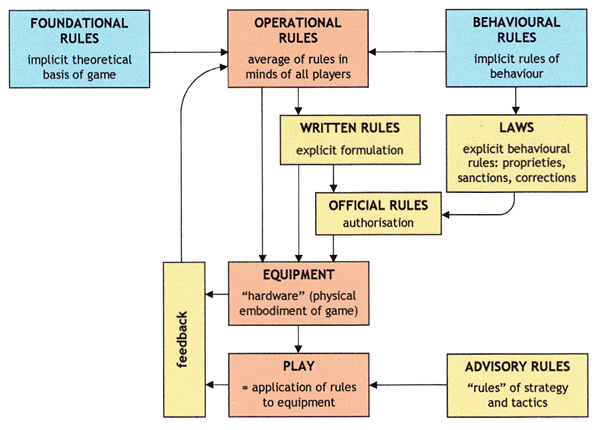
\includegraphics[width=8cm]{assets/rules.png}
    \caption{David Parlett's rule analysis\protect\footnotemark}
    \label{fig:rules}
\end{figure}
\footnotetext{\url{http://www.parlettgames.uk/gamester/rulesOK.html}, Accessed: 02-03-2018}

(1) Operational rules are everything a player needs to play a game.
They describe what is done to play the game.

(2) Foundational rules represent the underlying mathematical structure of the game.
Essentially breaking it down into states declaring when and how they change.


(3) Behavioral rules can be understood as the social contract when playing games.
Players intuitively understand these rules as fairplay which is why they are not written down.

(4) Written rules, in contract to behavioral rules, are explicitly manifested in documents that come with a game either physically or virtually.
Obtaining an understanding of the operational rules is achieved by reading the written rules, receiving explanations from others or simply by playing the game.
Due to the encoded nature of written rules most players tend to prefer different ways of learning.
They are exceptionally useful when players need to resolve conflicts and require a reference to neutral rules.

(5) Laws come into play during competitive tournaments.
They clarify or alter written rules and may include additional rules.
Modification or addition is mostly used to improve or balance games for serious scenarios.

(6) Official rules are the result of merging written rules and laws over time.
At some point they become the written rules again.

(7) Advisory rules assume a more strategic nature and boil down to advices helping players to perform better in a game.

(8) House rules are not included in Figure \ref{fig:rules} but are the result of the feedback loop.
Players may create their own set of rules to overcome deficiencies or to increase perceived fun.

Games are able to switch between different rule sets using modes.
Different modes alter parts of the existing rules or create sub-games with entirely new rules.
As players can get lost in these alternative modes they should be informed which mode is active and should not spend more time outside the main mode than inside.

Traditionally rules have been enforced by players or neutral referees in serious tournaments.
Computers can host much more complex games and automate the role of enforcing rules.
While this is powerful for creating rich games designers need to ensure that rules are intuitive for players.
Games should be designed in a way which allows players to test which things work and thereby discover rules naturally.

Cheating is the sole reason games require an enforcing instance for its rules.
Circumventing rules puts a player into a position of disproportional advantage which clearly satisfies the need for winning.
While this is a strong argument for enforcing rules already there is a more subtle effect at play as identified by \citeauthor{Schell2014}.
If a game is perceived as cheatable, whether that is actually the case or not, players might simply stop playing.
Investing time, effort and skill to work within the rules is rendered worthless by imagining someone potentially skipping these constraints.

Special attention should be payed to defining the main objective of a game. 
It can be considered the most important rule of all as it spurs motivation in players to achieve the defined goals \cite{Schell2014}.
Clearly defining all goals and how they relate to each other is essential for conveying the gist of a game in a well defined manner.
Only when players understand the objectives and are able to imagine ways ultimately achieving them they will feel an urge to play.
Three characteristics are shared by well-defined goals, they are: (1) Concrete, (2) achievable, and (3) rewarding.
It should be noted that these characteristics are not strict requirements and that they do not always have to be in perfect equilibrium.
Games can certainly be build around the exploration and discovery of the main objective (e.g. The Stanley Parable).
The same principle applies to achievable goals for a range of games centered around frustration and requiring excellent coordination to solve objectives (e.g. QWOP, Dark Souls series, Super Meat Boy).
Instead of players expressing resentment they manage to trigger an even stronger reverse effect of numerous attempts to beat the game.
This might be due to the goal still being concrete (e.g. finish all levels) and the perceived reward seeming particularly special as only a few players manage to finish these games.

\subsubsection{Skill} \label{sec:skill}
\textit{Skill} is a mechanic which games demand from players.
Matching a game's difficulty with the player's skill set creates a challenge; otherwise the game will be perceived as being too easy or too hard.
Naturally, more than a single skill is expected from players which generally stems from three main categories \cite{Schell2014}:

\begin{enumerate}
    \item \textbf{Physical:} Strength, dexterity, coordination, and physical endurance
    \item \textbf{Mental:} Memory, observation, puzzle solving, and decision making
    \item \textbf{Social:} Reading opponents, fooling opponents, communication, and coordination within teams
\end{enumerate}

It is important to stress that these skills refer to real-world abilities.
Whereas videogames often feature virtual character skills these a merely attributes which can be improved by providing the correct input to the game.
Nonetheless, this requires a level of physical coordination for using the input device and following a strategy allowing to improve virtual skills (cognitive work).

Actually defining the required skills for a game is useful to reflect about the design but also proves to be surprisingly difficult.
It is easy to think that a single skill is essential for performing well in a game.
In reality many factors are in play deciding which final blend of skills are actually necessary.
They can deviate far from what a designer might envision initially.

\subsubsection{Chance}
The final game mechanic \textit{chance} exerts a strong influence on all previously discussed mechanics.
There are many games not relying on chance as a game element, for example chess.
While players can only assume what the next move of their opponent will be (with the exception of \textit{zugzwang}) there is no uncertainty involved in actually executing moves.
Virtually every possible move could be calculated and pre-planned at any given point in time.
Introducing chance into games changes this property which in its essence leads to surprises \cite{Schell2014}.
With uncertain outcomes in games skills (Section \ref{sec:skill}) and chance start to influence each other.

Firstly, the ability to estimate chances is a mental skill.
Understanding and keeping track of probabilities through the course of a game can greatly improve the advantage of a player.
It does not equal perfect prediction of the future but if a player is aware of probabilities a successful outcome is much more likely.

Furthermore, skills themselves underlie probabilities meaning that every action involves risk.
Circling back to the example of chess not exhibiting randomness this changes when taking the perspective of a player.
Basic actions like moving a piece on the chess board are not affected by uncertainty whereas strategic actions definitely involve risk and a chance of success.
Trying to lead the opponent into a desired situation can go unnoticed with a certain probability which depends on the opponent's skill level.

Consequently, the ability to assess an opponent' skill is a mental skill too.
It is crucial for making decisions which course of action to take which depends on chances of success.
As a form of emergent behavior it can be useful for players to trick opponents into assuming a lesser or greater skill level than what they are actually capable of.

Players need to remember that predicting the chance of independent events is a purely imagined skill \cite{Schell2014}.
This behavior is commonly exhibited in the ``luck streak fallacy'' and ``gambler's fallacy''.
The second fallacy already suggests that this mistake is usually made in gambling games where the chance of an event stays the same (e.g. Roulette, whether the ball lands in black or red).
Game designers can try to take advantage of these fallacies to steer players towards making the desired choices.
Likewise, the assumption that pure chance can be influenced is false.
At the same time it is important to understand that if a game of pure chance is broken down to a series of isolated events which cannot be influenced most players will not experience fun.

\subsection{Story} \label{sec:story}
Historically speaking, story and gameplay have been two separate things.
Stories follow a single narrative whereas games can host groups of players and lead to different outcomes.
With the introduction of computer games to mainstream entertainment the lines between story and interactive gameplay started to blur.
Effectively challenging the assumption that they cannot be combined in its grounds.
Naturally, there are still ongoing debates about the interplay of story and gameplay.
Shifting the focus to published games shows that they consistently feature story elements of various kinds.
There are games which are build around a strong story line and in contrast less obvious stories intended for discovery and self-exploration.
\citeauthor{Schell2014} boils this combination down to a tool which helps to create and shape experiences.
The author explicitly stresses the similarity between traditional storytelling and its interactive variant.
They are not inherently different as both induce a desire to take action in listeners.
However, the latter actually enables listeners to participate and storytellers have to account for different narrative branches.
The following section discuss methods (\ref{sec:story-methods}) for story creation, common problems  (\ref{sec:story-problems}), guidelines for better stories  (\ref{sec:story-design}), and finally indirect control methods to create the feeling of freedom  (\ref{sec:story-freedom}).

\subsubsection{Methods} \label{sec:story-methods}
Interactive storytelling in games is mainly governed by two methods: (1) String of pearls and (2) story machine.

\textit{The string of pearls} (also known as \textit{rivers and lakes} \cite{Schell2014}) method presents a rather non-interactive story along its string.
Choosing techniques to present the story is hereby up to the game designer and can be realized in text, images or animated scenes.
Pearls along the string of story are sequences where players take full control.
They feature one or more goals with one final objective which upon completion progresses the story.
It is commonly criticized for seeming pseudo-interactive but in reality it provides players with a carefully crafted story with periods of interaction and freedom in between.
According to characteristics of interesting goals (Section \ref{sec:mechanics-rules}) the reward for finishing an interactive sequence is clearly the continuation of the story followed by more challenges.

In contrast to a pre-defined story the second method \textit{the story machine} postpones story generation until a game is played.
Good stories can be broken down into a sequence of interesting events \cite{Schell2014}.
Therefore, good games are essentially story machines producing series of events forming an interesting narrative.
This implies that designers are not necessarily defining the heart of these stories ahead of time nor are they in control of what players will actually experience.


\subsubsection{Problems} \label{sec:story-problems}
Creating interactive story trees is rather simple if qualities such as suspense, coherence, and enjoyment are ignored.
The special properties of branched narratives and the very nature of videogames in regards to reality introduce a range of obstacles.
\citeauthor{Schell2014} explores five of these problems in detail:

\begin{enumerate}
    \item \textbf{Unity:} Stories start out with a main problem in the beginning and finish with touching upon this again in the end (most of the time solving the problem). This introductory problem is the force pushing along the story. If players are able to deviate from this or avoid it entirely writing multiple endings with unity in respect to the beginning becomes an immense challenge. Consequently, interactive stories may loose their strength and feel disconnected to the beginning.
    \item \textbf{Combinatorial explosion:} Each choice leading to unique outcomes contributes to the exponential growth of branches within a story. Increasing the depth of branching leads to an excessive amount of story lines. Ensuring quality for every different outcome is not feasible anymore. As a remedy to this problem branches can be merged together again. However, this creates a chain of compromises ultimately rendering the choices meaningless as they lead to a common ending.
    \item \textbf{Multiple endings disappoint:} At first it may seem like providing players with multiple endings creates a rich game. Playing it again will yield a different experience. However, players commonly find themselves questioning whether they took the right path. This is due to alternative endings not having the same level of unity with their beginning. Furthermore, players will dread missing out on other endings and being required to complete the story once again.
    \item \textbf{Not enough verbs:} Activities in videogames vastly differ what characters in book or movie stories are doing. While game technology has seen immense improvements in terms of fidelity recreating natural conversations still feels rather restricted. Stories heavily rely on communication between characters. Progress in the field of artificial intelligence can potentially counteract this problem.
    \item \textbf{Time travel:} Compelling stories usually feature tragedy and inevitability. It is challenging for games to support freedom and control while also supporting inevitability. If the player controls a story's main character, for example, any death will will revert time to the last checkpoint. Designers may choose to increase the punishment by resetting the player further or even to the beginning but this mechanic does not recreate tragic. Nevertheless, sophisticated design is able to circumvent this problem. Examples can be found in the story-driven ``The Walking Dead'' or ``The Wolf Among Us'' games by Telltale Games. Choices of players influence the story in drastic and final ways; going as far as progressing without dead characters.
\end{enumerate}

\subsubsection{Design Guidelines} \label{sec:story-design}
The previously enumerated problems create the impression that interactive storytelling can hardly produce compelling experiences.
\citeauthor{Schell2014} argues that moving the focus from stories back to experiences thereby adjusting expectations should be the goal.
Using traditional storytelling with game mechanics can create unexpected and innovative experiences.
The author suggests nine different guidelines which help to streamline the creation of better game experiences:

\begin{enumerate}
    \item \textbf{Goals, obstacles, and conflicts:} Following the main paradigm of movie storytelling two components play key roles: Characters with goals and obstacles interfering in reaching these goals. Conflicts emerge when other characters aim to achieve contrasting goals. The same principle applied to videogame stories leads to: Players engaging in problem solving and conflicts creating surprising outcomes. Nonetheless, games need to align goals and obstacles with their story. Otherwise they may feel superfluous and have a detrimental effect on the overall experience.
    \item \textbf{Backstory:} While elaborate backstories found in books and movies might not be necessary virtual worlds should have enough support to feel real. They certainly need to feel real for game designers in order to convey this idea to players. Motivation of characters should be grounded in the history of the world.
    \item \textbf{Simplicity and transcendence:} Virtual worlds are simpler than reality while also making the player more powerful than in reality (transcendence). This combination proves to be successful as it allows players to sufficiently understand the virtual world and equips them with the ability to achieve their goals.
    \item \textbf{The hero's journey:} Joseph Campbell describes a common structure of heroic stories in his book. Christopher Vogler turns these fundamentals into a practical guide for creating heroes according to Campbell's identified pattern. Due to the heroic nature of many videogame stories these works are a natural fit for structuring compelling stories.
    \item \textbf{Adapt the story:} It is common to venture out on game design by solely focusing on the story first. This can neglect other essential parts which are often more expensive to change. Balancing gameplay requires fine tuning of mechanics and adaption of technology results in complex reprogramming. Instead of changing rigid game components it might be possible that rewriting specific parts of the story is an easier solution.
    \item \textbf{Consistency:} Game worlds are intricate, fragile constructs which rely on consistency. Only if a world is consistent to itself, meaning that universal rules apply to everything in the same way, players are able to immerse themselves. Even one logical error can initiate the disintegration of the game world as a construct.
    \item \textbf{Accessibility:} Games feature elements that are not necessarily accurate in respect to reality for the benefit of what players will believe and enjoy. It is important to keep surreal and inaccurate elements in mind and finding a way to weave them into the world. Players will accept an unusual world as long as the elements inside are natural to this scenario.
    \item \textbf{Balancing the use of clich\'es:} Designers need to find the right balance between avoiding clich\'es at all costs and overusing them. As a middle ground combining familiar elements with novel additions is a sensible approach. It might provide players with a known clich\'e while introducing something new to build upon.
    \item \textbf{Maps as story elements:} Whether a game occupies a physical space or is described in words, creating maps helps both designers and players to visualize the world. Stories can be draped around the shape of these maps. This approach often leads to natural stories as designers have to think about the actual layout of their worlds.
\end{enumerate}

\subsubsection{Feeling of Freedom} \label{sec:story-freedom}
At its core the clash between story and gameplay is about feeling or more specifically the sense of freedom \cite{Schell2014}.
The power of control is crucial for interactive experiences it allows players to immerse themselves in a world where they are actually able to act in steered by their imagination.
This indicates handing over full control to the player which would create problems discussed in Section \ref{sec:story-problems}.
Meanwhile, giving the player a feeling of freedom is a powerful hybrid combining the advantages of a carefully crafted story and the perceived freedom of choice.
This is made possible by applying indirect control methods to the actions of players:

\begin{enumerate}
    \item \textbf{Constraints:} Restrictions on the number of choices retain the freedom of choice while also preventing cognitive overload through a sheer number of options. There is still uncertainty which option the player chooses but it will ultimately be from the set of pre-defined choices.
    \item \textbf{Goals:} Previously discussed as the central driving force in Section \ref{sec:mechanics-rules} goals are also inherently useful to steer players towards activities connected to these goals. It is thereby only necessary to provide content surrounding these goals. Adding extra content for secondary goals helps to maintain the feeling of freedom while most players will stick to the primary route.
    \item \textbf{Interface:} Both physical and virtual game interfaces are able to exert indirect control on the activities a player might choose. Designing these interfaces with desired activities in mind lowers the probability of players going alternative paths.
    \item \textbf{Visual design:} Drawing attention to different parts of a game's layout allows indirect control on what player's are most likely going to look at. Subsequently, this helps to control where a player might be headed to.
    \item \textbf{Characters:} Non-player characters (NPCs) are especially useful to control the actions of players. Different ways of emotional connections with NPCs decide whether a player obeys, protects, helps or tries to defeat them. It should be noted that this mechanism only works if players empathize with an NPC or have an emotional response.
    \item \textbf{Music:} While music is a great tool to create a desired atmosphere and vibe in games it also acts on the emotional mood of players. The speed, energy and type greatly influences the general feeling of players and can help to steer them along the story.
    \item \textbf{Collusion:} Assigning two goals to NPCs enables them to partake in creating interesting gameplay or stories. Aside from serving their main purposes one of their goals is to assists the designer in ensuring an optimal game experience of the player. This can unravel in NPCs leading players to interesting places or maintaining an optimal tension pattern in the story.
\end{enumerate}
\section{MTDA+N Framework} \label{sec:mtda+n}
Ralph and Monu (2014) \cite{Ralph2014} base their article on the MDA framework (Section \ref{sec:mda}) and the elemental tetrad (Section \ref{sec:elemental-tetrad}).
They recognize both frameworks as useful tools for reasoning about game design and being commonly cited in research.
Nonetheless, relying on two separate works is inefficient as they share redundancy.
Integrating these frameworks serves the purpose of working towards a unified game theory covering all relevant areas adequately.
Mechanics and aesthetics are present in either model and the authors generally describe similar ideas.
Technology from Schell's elemental tetrad \cite{Schell2014} and dynamics MDA by Hunicke et al. \cite{Hunicke2004} are also transferred into the integrated framework.

\subsection{Narrative}
According to the authors of MTDA+N the term story carries too much overloaded meaning and is not necessarily suitable for many games lacking traditional stories (e.g. Tetris).
Instead they propose the term narrative which is categorized into three distinctive types.
They will be discussed in the following sections.

\subsubsection{Embedded Narrative}
An embedded narrative is actual content of the game itself.
It is told by the game designers through in-game mechanisms like cutscenes, audio dialogue or graphic artwork.
This fits very well with the string of pearls method discussed by \citeauthor{Schell2014} (Section \ref{sec:story-methods}).
The embedded narrative would take place in between the pearls along the string.

\subsubsection{Emergent Narrative}
In contrast to the embedded narratives the \textit{emergent} variant is only created when players actually use the game.
The name already suggests that the narrative emerges as players take part in the game world.
Certain actions can trigger a chain of events which in turn created sequences of interesting events.
Games acting as story machines (Section \ref{sec:story-methods}) are essentially producing emergent narratives governed by the behavior of players.
Players are effectively responsible for emergent narratives and stories are dependant on how they perceive events in the game.

\subsubsection{Interpreted Narrative}
Players are constantly interpreting both embedded and emergent narratives.
This interpretation is not part of the game itself but rather resides in the mental representation in a player's mind \cite{Ralph2014}.
Therefore, the interpreted narrative acts on the level of aesthetics and influences the experience of a game.

\subsection{Model}
Finally, merging the MDA framework (Figure \ref{fig:mda}) and elemental tetrad (Figure \ref{fig:elemental-tetrad}) results in the \textit{Mechanics, Technology, Dynamics, Aesthetics plus Narratives} framework (MTDA+N) depicted in Figure \ref{fig:mtda+n}.

\begin{figure}[H]
    \centering
    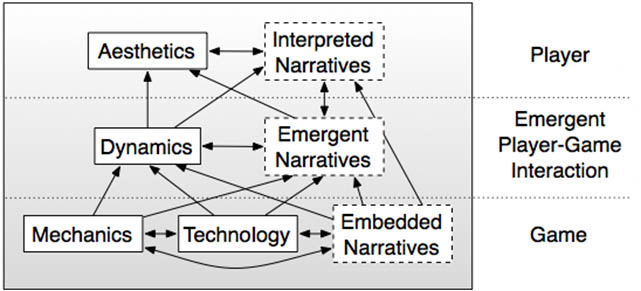
\includegraphics[width=8cm]{assets/mtda+n.jpg}
    \caption{MTDA+N framework\protect\footnotemark}
    \label{fig:mtda+n}
\end{figure}
\footnotetext{\url{http://www.firstpersonscholar.com/a-working-theory-of-game-design}, Accessed: 02-03-2018}

Player primarily interact with mechanics and experience the embedded narrative.
These interactions result in behavioral dynamics of the game and potentially unravels emergent narratives.
Finally, aesthetics and the interpreted narrative reside in the player's mental state and essentially form the experience.

\section{Artificial Intelligence in Games} \label{sec:ai}
In their paper Yannakakis and Togelius (2015) \cite{Yannakakis2015} establish a taxonomy of ten different fields within artificial intelligence (AI) in games.
This overview helps to gain an understanding of the current research state and highlights interaction between fields.
Furthermore, it emphasizes potential interconnections which bear the potential to progress connected fields if further explored.

\subsection{NPC Behavior Learning} \label{sec:npc-behavior-learning}
Teaching non-player characters (NPCs) to perform well in a game can be understood as a reinforcement problem.
Naturally, games feature measurements (e.g. score, time) useful for determining whether a learning algorithm is performing good.
The field of NPC behavior learning influences other AI areas to a large extent: Player modeling aims to mimic the style of players which benefits from the same learning algorithm, better NPC AI algorithms push the development of new game benchmarks matching their performance, and testing of procedural generated content can be automated by using capable AI.

\subsection{Search and Planning} \label{sec:search-and-planning}
Search algorithms from computer science are commonly applied to pathfinding problems or searching the decision space of games with a high magnitude of branching.

Porteous et al. (2010) \cite{Porteous2010} introduce an interesting application of planning on interactive storytelling (Section \ref{sec:story}).
Their AI planning aims to solve narrative generation using novel state constraints.
It overcomes the issue of controlling the shape of generated narratives using these constraints while also maintaining real-time performance.
Consequently they defined the following requirements for planning in interactive storytelling, planners need to: (1) Perform in real-time, (2) derive planning criteria from constraints, (3) support interactivity, and (4) are able to reason about narrative knowledge.
Building the planning around domain-specific knowledge helps to solve problems in a more efficient manner.
Specifying constraints around this domain allows authors to control which situations are crucial for the narrative.
Firstly, a baseline linear plot is constructed along with a set of basic, generic actions (planning operators).
Each character has a different point of view (PoV) and a varying set of available actions.
Identifying the plot for each character in respect to PoV and actions transformed the basline into a nonlinear plot.
Interacting with the narrative changes facts about the worlds which triggers the engine to search for different storylines according to the declared constraints.

\subsection{Player Modeling}
The field of player modeling is concerned with creating machine learning (ML) models detecting how players experience games and their resulting emotional change.
Identifying archetypes of players is then an example application of unsupervised clustering to detect groups.
Being able to model players is beneficial for both procedural content generation and computationally generated narratives to create personalized content and scenarios.

\subsection{Games as AI Benchmarks}
When games or parts of them are used as benchmarks they provide an interface which allows external systems to measure the performance of the AI under test.
Commonly annual or ongoing competitions are held around AI benchmarks pushing development in the field.
Benchmarks are an essential tool to measure and compare the performance of competing AI systems.
It is therefore crucial to build quality benchmarks to progress the research of AI in games as a whole.
However, creating too narrow benchmarks involves the risk of focusing effort on specific problems.
Instead AI should become better at solving general problems.

\subsection{Procedural Content Generation}
Procedural content generation (PCG) is concerned with the automatic or semi-automatic generation of any game content.
Among others, generating levels or stories are only two examples for PCG.
There is a close interconnection between PCG and the field of NPC behavior learning (Section \ref{sec:npc-behavior-learning}).
In order to generalize well and perform good in unseen environments AI controlled NPCs can used procedural generated levels to test their abilities.
Using automated NPCs to play generated levels is in turn a way to check if a level is solvable.

\subsection{Computational Narrative}
Representational and generational aspects are part of the computational narrative.
Stories are essential for shaping the aesthetics of a game.
The main questions of this field revolve around how to represent narratives and how AI can take part in generating their sequence.
As discussed in the paper by Porteous et al. \cite{Porteous2010} planning influences computational narrative.
It enables the generation of multiple variants while obeying constraints defined by the story authors.

\subsection{Believable Agents}
Any game featuring NPCs is usually interested in improving the believability of its agents.
They have to express certain human-like characteristics towards players in order to be taken seriously.
Prominent competitions like the 2k BotPrize are essentially turing tests for imitating gameplay of human players.
The commercial game industry is especially interested in creating more believable agents as it allows for more immersive virtual worlds.

\subsection{AI-assisted game design}
The area of AI-assisted game design carries potential for progression of the field and creating benefits for other research areas.
It focuses on the development of AI-powered tools assisting in the design and development process of games.
Specifically the creation of levels, complete maps, mechanics and narratives can be supported by AI tooling.

\subsection{General Game AI}
Researchers have established the field of artificial general intelligence (AGI) in recent years which aims to progress AI towards human-level domain-independent intelligence.
Similarly game playing AI agents should be capable to play various kinds of games with only an initial learning phase.
The annual General Game Playing Competition tests agents on rather restricted variants of games with perfect information and discrete state.
Progress has been made to test agents on 2D videogames which are described using the Video Game Description Language specifically designed for this purpose.

\subsection{AI in commercial games}
There are disjoint efforts between academic research and the commercial game industry when working on AI in games.
This is partly due to each group being interested in solving different problems.
Researchers are focused on general, deep problems whereas commercial games only require AI for improving the player's experience.
However, it would be beneficial for both groups to work towards closing this gap.
The use of AI in commercial games provides constant input for research and AI techniques from academia have regularly found application in published, successful games.

\section{Conclusion}
This paper highlights the challenge of establishing a unified game design framework.
Games consists of numerous moving parts which constantly influence each other.
As they continue to become more complex these interconnections grow as well.
Designers need to be able to decompose games in an abstract way in order to understand different components and how they contribute to the final experience.
The authors of MTDA+N manage to integrate the two previous design frameworks (MDA and the elemental tetrad) while also further exploring the narrative component.
However, they are aware that it still does not cover all areas of games adequately.
For example the role and nature of the player is mostly disregarded in their model.
Artificial intelligence is also lacking in the common game design frameworks.
The various research fields bear potential for all areas of game design.
Especially challenges in interactive storytelling can be tackled differently using AI technology.

\bibliographystyle{ACM-Reference-Format}
\bibliography{Mendeley}

\end{document}
